%%%%%%%%%%%%%%%%%%%%%%%%%%%%%%%%%%%%%%%%%
% University/School Laboratory Report
% LaTeX Template
% Version 3.1 (25/3/14)
%
% This template has been downloaded from:
% http://www.LaTeXTemplates.com
%
% Original author:
% Linux and Unix Users Group at Virginia Tech Wiki 
% (https://vtluug.org/wiki/Example_LaTeX_chem_lab_report)
%
% License:
% CC BY-NC-SA 3.0 (http://creativecommons.org/licenses/by-nc-sa/3.0/)
%
%%%%%%%%%%%%%%%%%%%%%%%%%%%%%%%%%%%%%%%%%

%----------------------------------------------------------------------------------------
%	PACKAGES AND DOCUMENT CONFIGURATIONS
%----------------------------------------------------------------------------------------

\documentclass{article}

\usepackage[version=3]{mhchem} % Package for chemical equation typesetting
\usepackage{siunitx} % Provides the \SI{}{} and \si{} command for typesetting SI units
\usepackage{graphicx} % Required for the inclusion of images
\usepackage{natbib} % Required to change bibliography style to APA
\usepackage{amsmath} % Required for some math elements 
\usepackage[utf8]{inputenc}
\usepackage{tikz,pgfplots}
\usepackage[letterpaper, margin=0.5in]{geometry}
\usepackage{float}
\usepackage{enumitem}
\usepackage{gensymb}
\usepackage[hidelinks,bookmarks]{hyperref}
\usepackage[all]{hypcap}
\usepackage{subfloat}
\usepackage{color}
\usepackage{listings}

% Roman numerials
\pagenumbering{arabic}

\setlength\parindent{0pt} % Removes all indentation from paragraphs

%\renewcommand{\labelenumi}{\alph{enumi}.} % Make numbering in the enumerate environment by letter rather than number (e.g. section 6)

%\usepackage{times} % Uncomment to use the Times New Roman font

% for some tables
\newcommand{\specialcell}[2][c]{%
  \begin{tabular}[#1]{@{}c@{}}#2\end{tabular}}
  
\newcommand{\me}{\mathrm{e}}
\providecommand{\e}[1]{\ensuremath{\times 10^{#1}}}

\newcommand{\eqname}[1]{\tag*{#1}}

\renewcommand{\labelitemii}{$\circ$}

\DeclareMathOperator\erfc{erfc}

%%%%%%%%%%%% COLOR DEFINITIONS %%%%%%%%%%%%%

\definecolor{silicon}{RGB}{255,102,102}
\definecolor{oxide}{RGB}{145,150,110}
\definecolor{ioxide}{RGB}{175,180,135}
\definecolor{goxide}{RGB}{195,200,150}
\definecolor{poly}{RGB}{155,20,155}
\definecolor{spinglass}{RGB}{200,205,100}
\definecolor{n+}{RGB}{250,15,15}
\definecolor{aluminum}{RGB}{30,30,30}

%----------------------------------------------------------------------------------------
%	DOCUMENT INFORMATION
%----------------------------------------------------------------------------------------

%\title{Determination of the Atomic \\ Weight of Magnesium \\ CHEM 101} % Title

%\author{John \textsc{Smith}} % Author name

%\date{\today} % Date for the report

\begin{document}

%\maketitle % Insert the title, author and date

% If you wish to include an abstract, uncomment the lines below
% \begin{abstract}
% Abstract text
% \end{abstract}

%----------------------------------------------------------------------------------------
%	SECTION 1
%----------------------------------------------------------------------------------------

\section{Measurements \& Parameter Extraction}

\subsection{Line Width/Misalignment}


\subsection{Four-Point Resistors [2a, 2b]} %%%%%%%%%%%%% Resistors 2a 2b

\subsubsection{Measurement Setup}
\begin{figure}[H]
\centering
\begin{tikzpicture}
\node at (5,5) {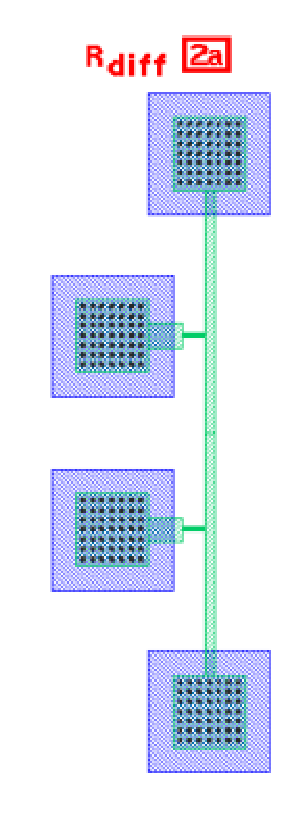
\includegraphics[height=250pt]{Device_setup/device2a1.pdf}};
\draw [<->,thick] (6,7.8) -- (8,7.8) -- (8,7.5); %SIM4
\node at (10,7.3) {V sweep, -0.1 to 0.1 V, comp 5, I measured};
\draw [<->,thick] (6,1.8) -- (8,1.8) -- (8,2.2); %Sim3
\node at (8,2.35) {GND};
\draw [<->,thick] (5,5.5) -- (7,5.5); %SIM1
\node at (9.5,5.5) {GND, comp 5, measure V};
\draw[<->,thick] (5,4) -- (7,4); %SIM2
\node at (9.5,4) {GND, comp 5, measure V};
\node at (15,5) {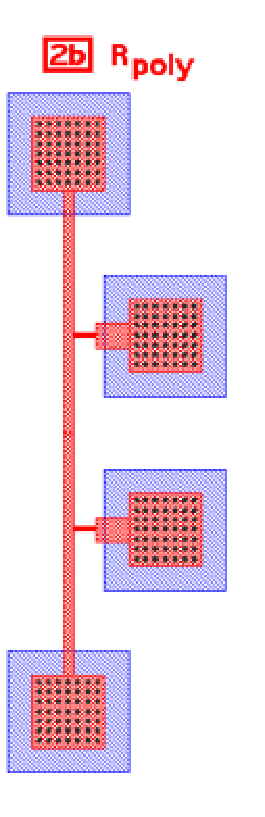
\includegraphics[height=250pt]{Device_setup/device2b1.pdf}};
\draw [<->,thick] (14,7.8) -- (8,7.8) -- (8,7.5); %SIM4
\draw [<->,thick] (14,1.8) -- (8,1.8) -- (8,2.2); %Sim3
\draw [<->,thick] (15,5.5) -- (12,5.5); %SIM1
\draw[<->,thick] (15,4) -- (12,4); %SIM2
\node at (5.2,7.8) {\textbf{A}};
\node at (4,4.7) {\textbf{VDiff}};
\draw[->,thick] (4.1,4.8) -- (4.2,5.1);
\draw[->,thick] (4.1,4.6) -- (4.2,4.4);
\end{tikzpicture}
\caption{Device 2a is a diffusion resistor and 2b is a poly resistor.}
\end{figure}

\subsubsection{I-V plot for the diffusion resistor, 2a}
\begin{figure}[H]
\centering
\begin{tikzpicture}
\node at (5,5) {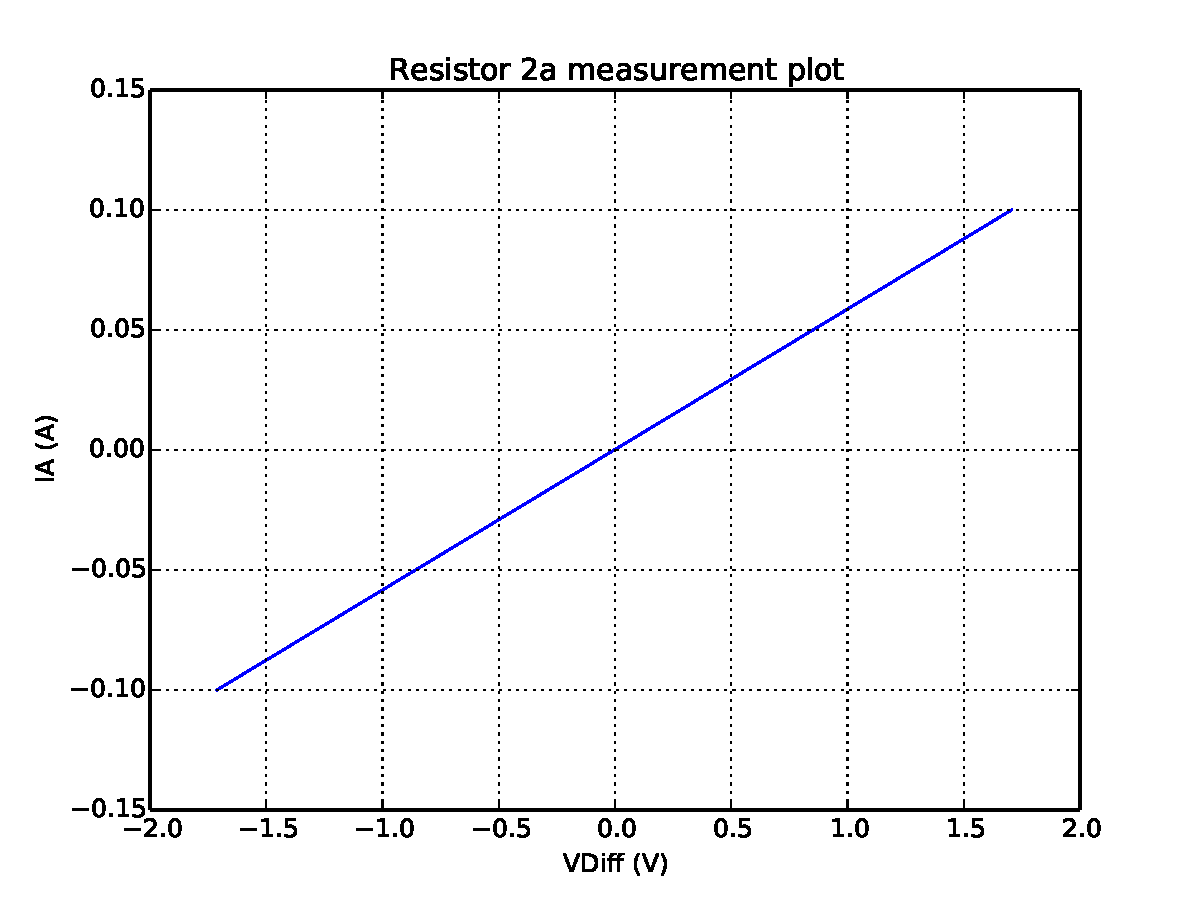
\includegraphics[width=250pt]{Device_plot_data/D2aplot.pdf}};
\end{tikzpicture}
\caption{A plot of the measurement data taken for resistor 2a. The plot is based off of 2 data points.}
\end{figure}

Get resistance, sheet resistance, doping concentration, electron mobility ....

\subsubsection{I-V plot for the poly resistor, 2b}
\begin{figure}[H]
\centering
\begin{tikzpicture}
\node at (5,5) {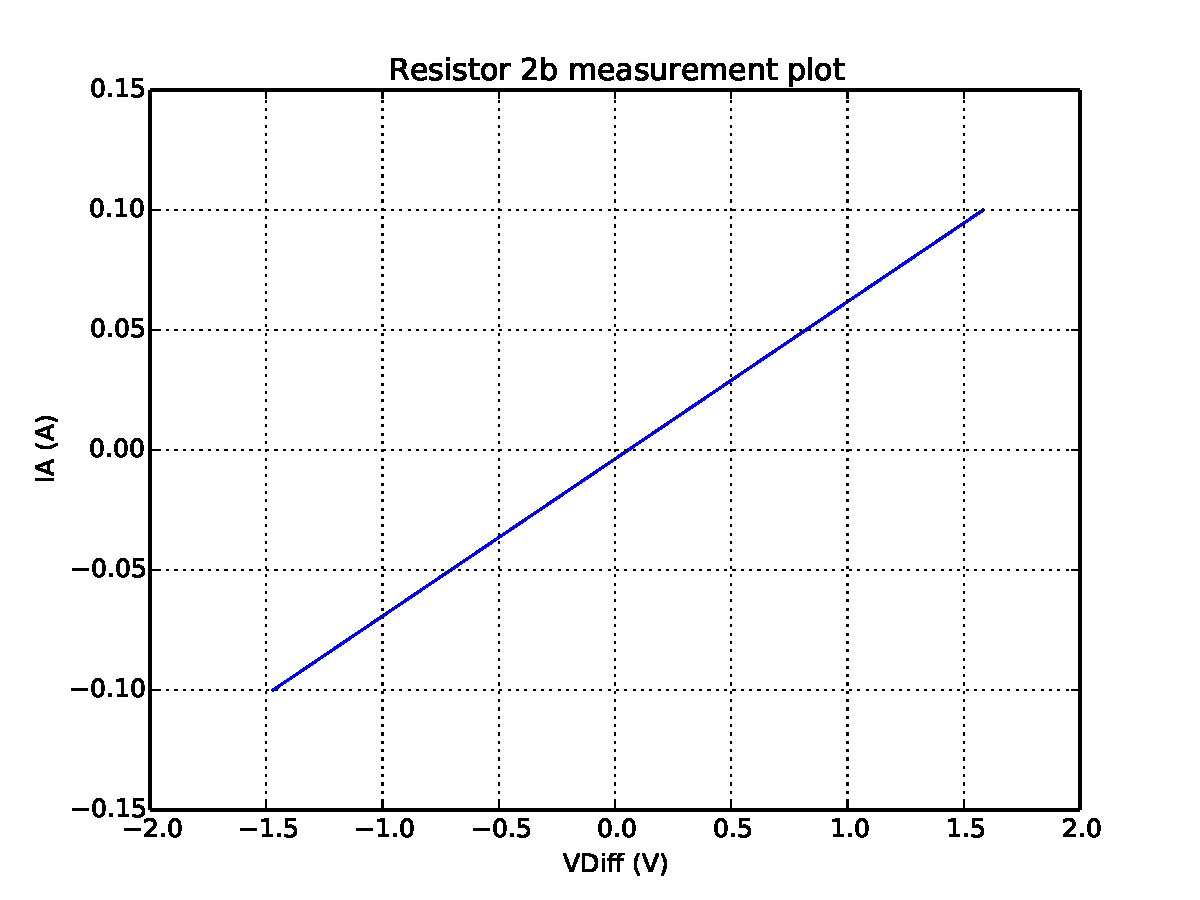
\includegraphics[width=250pt]{Device_plot_data/D2bplot.pdf}};
\end{tikzpicture}
\caption{A plot of the measurement data taken for resistor 2b. The plot is based off of 2 data points.}
\end{figure}

Get resistance and sheet resistance...


\subsection{Four-Point Contact-Chain Resistor [2c, 2d]} %%%%%%%% Resistors 2c 2d

\subsubsection{Measurement Setup}
\begin{figure}[H]
\centering
\begin{tikzpicture}
\node at (5,5) {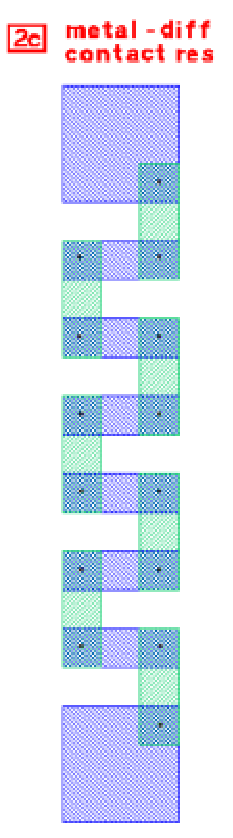
\includegraphics[height=250pt]{Device_setup/device2c2.pdf}};
\draw[<->,thick] (5,8) -- (8,8) -- (8,7); %Sim1
\node at (9,6.8) {V sweep, -5 to 5 V, measure I, V };
\draw[<->,thick] (5,1.5) -- (8,1.5) -- (8,2.5); %Sim2
\node at (8,3) {GND};
\node at (13,5) {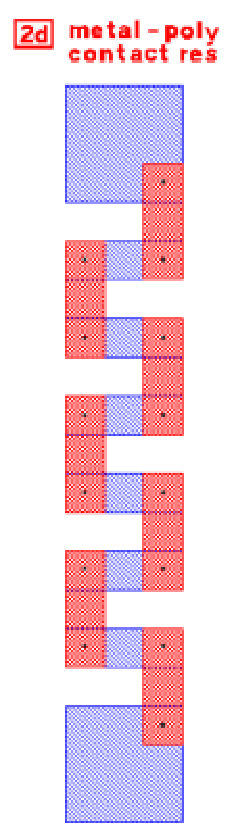
\includegraphics[height=250pt]{Device_setup/device2d2.pdf}};
\draw[<->,thick] (13,8) -- (8,8) -- (8,7); %Sim1
\draw[<->,thick] (13,1.5) -- (8,1.5) -- (8,2.5); %Sim2
\node at (4.8,8) {\textbf{A}};
\end{tikzpicture}
\caption{Chain resistor setup for diffusion and poly resistors.}

\end{figure}

\subsubsection{b. I-V plot for diffusion resistor, 2c}
\begin{figure}[H]
\centering
\begin{tikzpicture}
\node at (5,5) {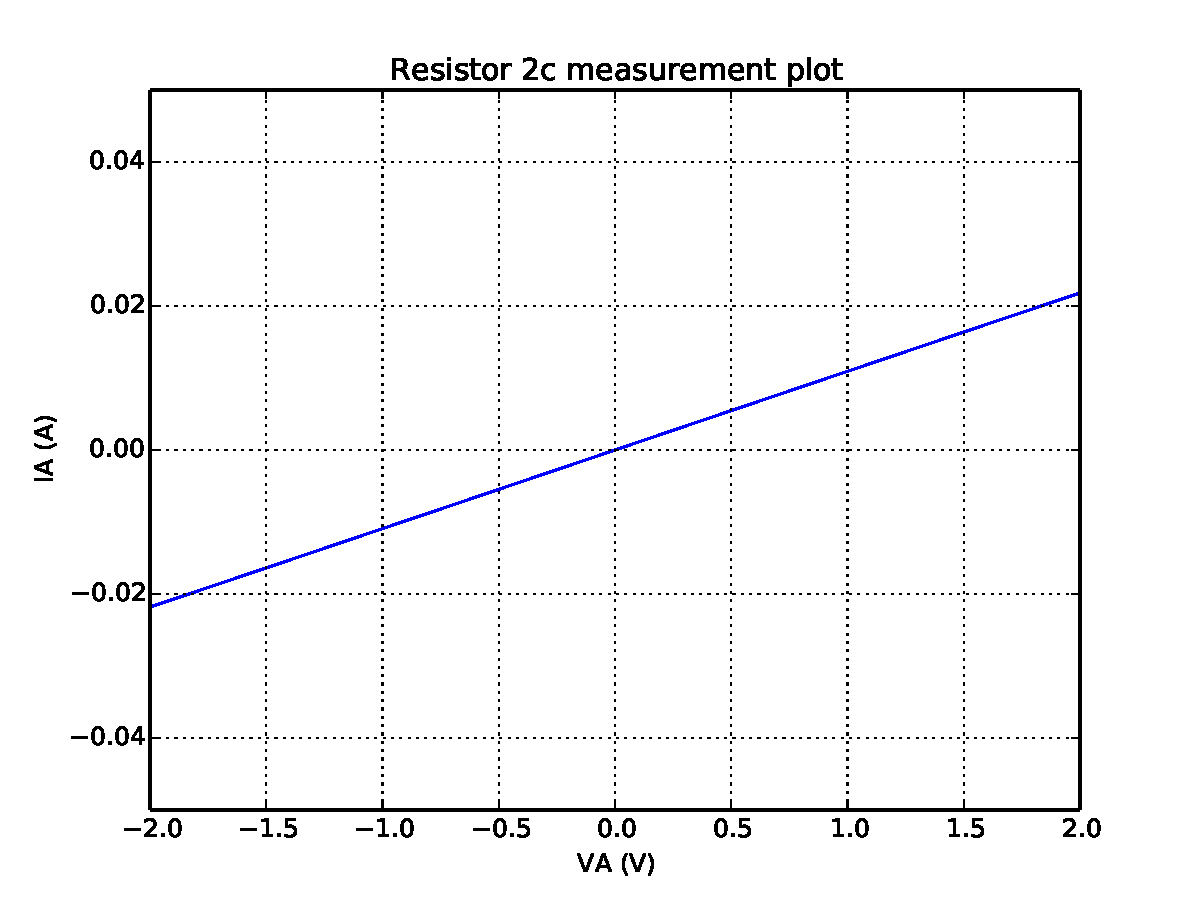
\includegraphics[width=250pt]{Device_plot_data/D2cplot.pdf}};
\end{tikzpicture}
\caption{A plot of the measurement data taken for resistor 2c. The plot is based off of 2 data points.}
\end{figure}


i. Extract the resistance \\
ii. Extract metal-to-diffusion contact resistance

\subsubsection{b. I-V plot for poly resistor, 2d}
\begin{figure}[H]
\centering
\begin{tikzpicture}
\node at (5,5) {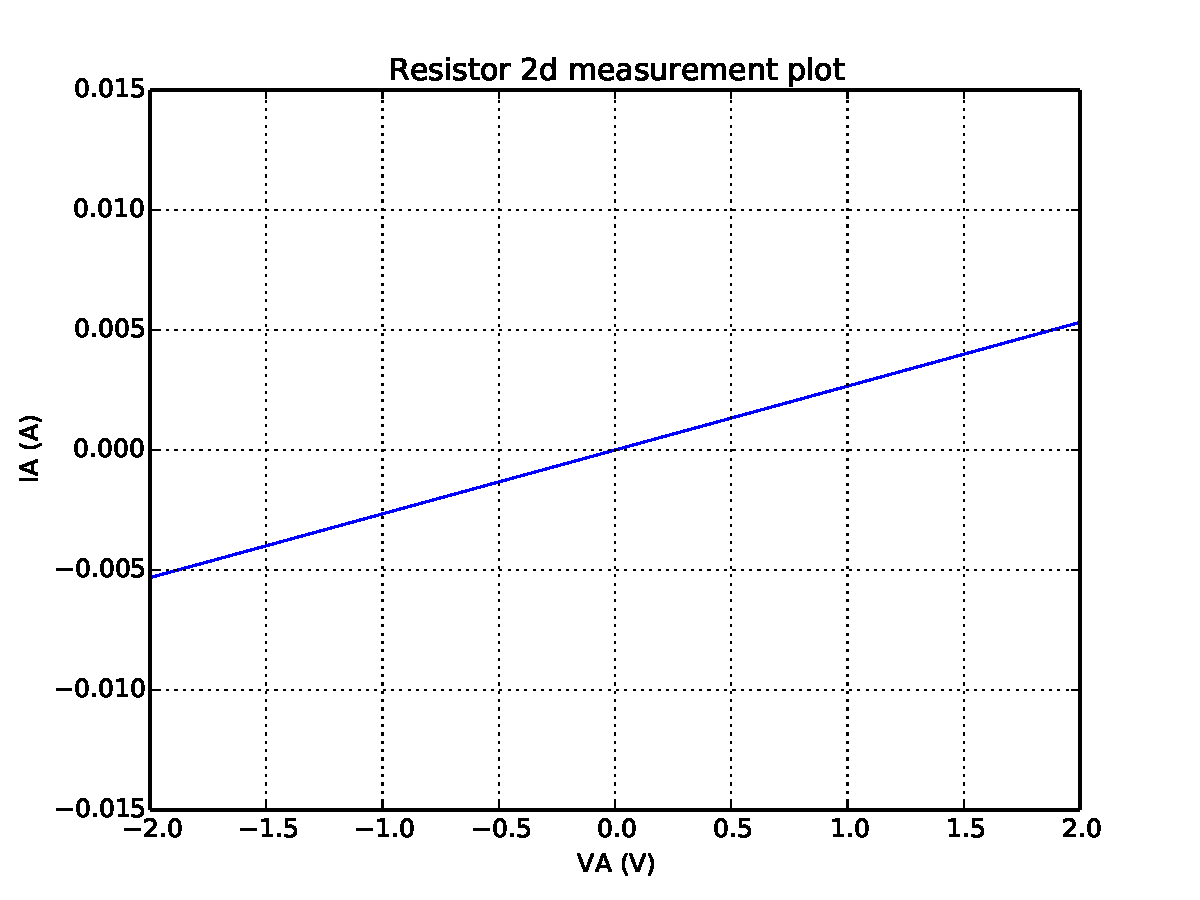
\includegraphics[width=250pt]{Device_plot_data/D2dplot.pdf}};
\end{tikzpicture}
\caption{A plot of the measurement data taken for resistor 2d. The plot is based off of 2 data points.}
\end{figure}

i. Extract the resistance \\
ii. Extract metal-to-poly contact resistance


\subsection{Gate Oxide Capacitor, 4} %%%%%%% Gate capacitor 4

\subsubsection{Measurement Setup}

\subsubsection{C-V plot of gate oxide capacitor w/ lights ON}
Minimum capacitance

\subsubsection{C-V plot of gate oxide capacitor w/ lights OFF}

minimum capacitance ...

\subsection{Field Oxide Capacitor, 3} %%%%%%% Field Oxide Capacitors 3

\subsubsection{Measurement Setup}

\subsubsection{C-V plot of field oxide capacitor}
Minimum capacitance

\subsubsection{Capacitance in the accumulation region}

minimum capacitance ...

\subsubsection{Field oxide thickness}

stuff...

\subsection{Intermediate Oxide Capacitors, 5} %%%%%%% Intermediate Oxide Capacitor 5

\subsubsection{Measurement Setup}

\subsubsection{C-V plot of intermediate oxide capacitor}

stuff ...

\subsubsection{Capacitance in the accumulation region}

stuff...


\subsection{Diode, 7} %%%%%%%%% Diode 7

\subsubsection{Measurement setups for forward and reverse operations}
\begin{figure}[H]
\centering
\begin{tikzpicture}
\node at (5,5) {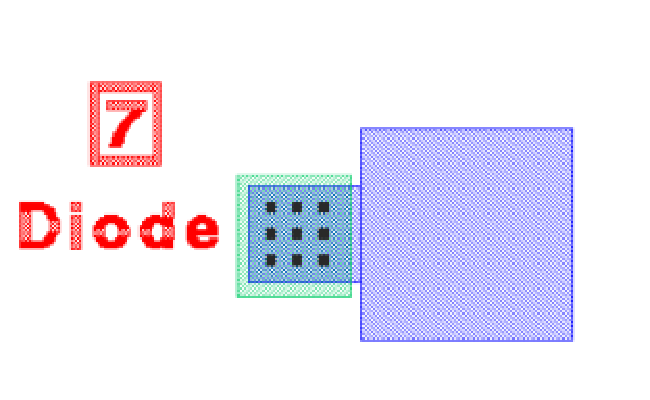
\includegraphics[width=200pt]{Device_setup/device7a2.pdf}};
\node at (15,5) {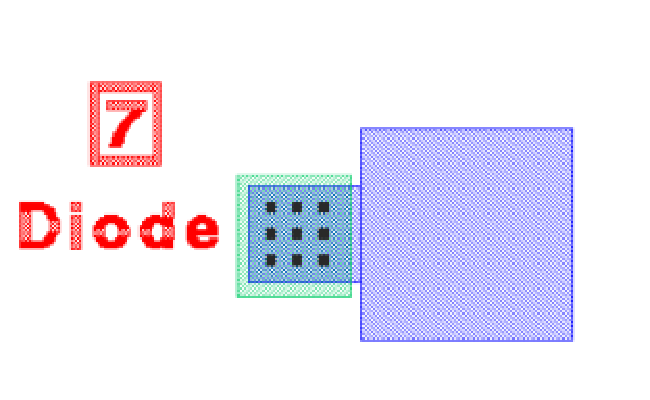
\includegraphics[width=200pt]{Device_setup/device7a2.pdf}};
\node at (6.5,4.5) {\textbf{A}};
\node at (16.5,4.5) {\textbf{A}};
\draw[<->,thick] (6,5) -- (9,5) -- (9,6);
\node at (9,6.2) {V sweep, -1 to 1 V, measure I, V };
\node at (5,3) {Stage connector set to GND};
\draw[<->,thick] (17,4.5) -- (17,3.6) -- (13,3.6) -- (13,3.2);
\node at (13,3.0) {V sweep, -40 to 40 V, comp 0.05, measure I, V };
\node at (13,2.5) {Stage connector set to -40 V, comp 0.05};
\node at (5,7) {\textbf{Test 1 (forward)}};
\node at (15,7) {\textbf{Test 2 (reverse)}};
\end{tikzpicture}
\caption{Two tests were performed on this diode; both measurement setups are shown above.}
\end{figure}

\subsubsection{I-V plots for forward and reverse operation}
\begin{figure}[H]
\centering
\begin{tikzpicture}
\node at (5,5) {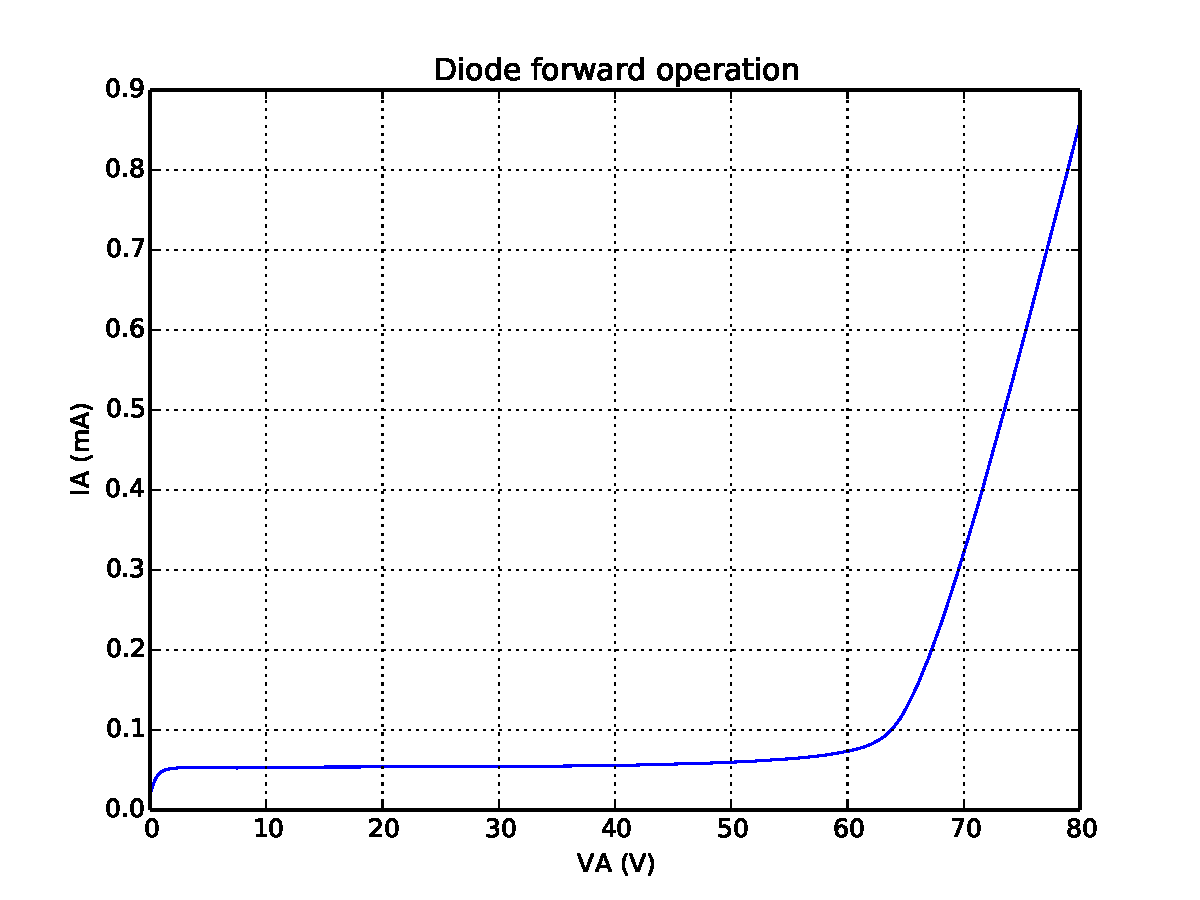
\includegraphics[width=250pt]{Device_plot_data/D7aplot.pdf}};
\node at (15,5) {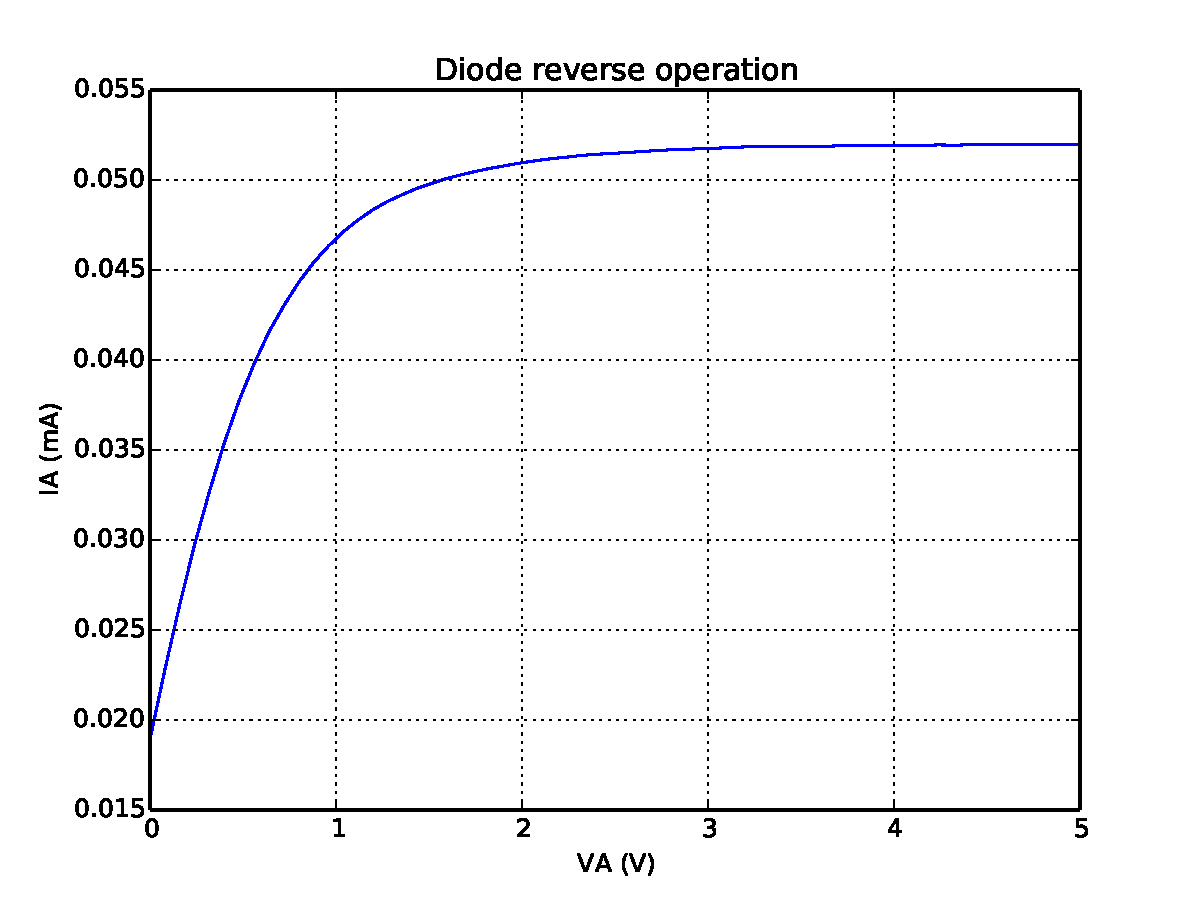
\includegraphics[width=250pt]{Device_plot_data/D7bplot.pdf}};
\end{tikzpicture}
\caption{Plots of forward and reverse operation of Diode 7.}
\end{figure}

\subsubsection{Extract the turn-on voltage and the series resistance}


\subsection{MOSFETs of Varying Length, [8a-d]}

\subsubsection{Measurement setups}
\begin{figure}[H]
\centering
\begin{tikzpicture}

\node at (5,5) {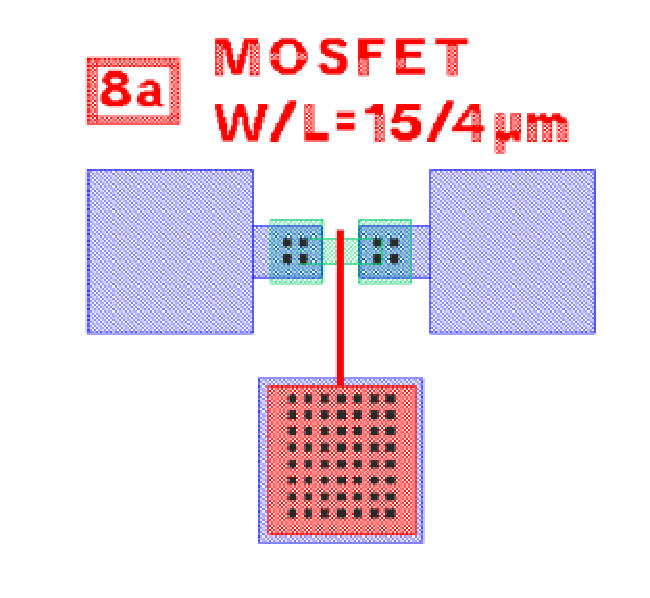
\includegraphics[width=200pt]{Device_setup/device8a2.pdf}};
\node at (15,5) {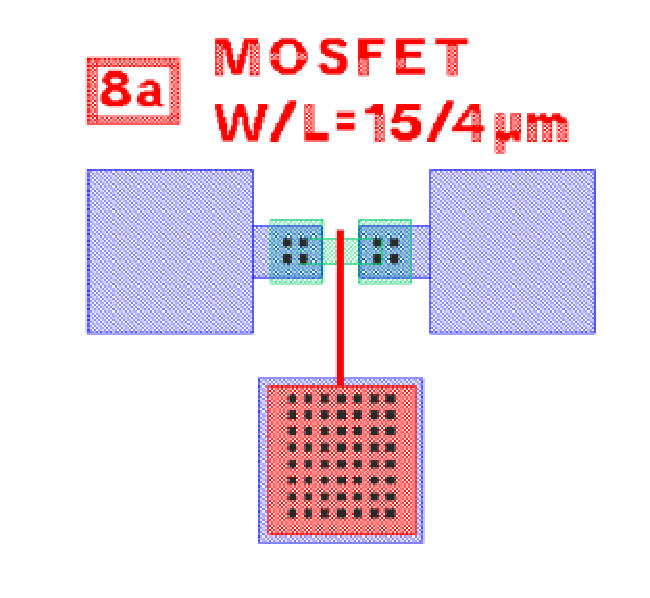
\includegraphics[width=200pt]{Device_setup/device8a2.pdf}};
\node at (5,9) {\textbf{Test 1}};
\node at (15,9) {\textbf{Test 2}};
\node at (3.5,6) {\textbf{D}};
\node at (7,6) {\textbf{S}};
\node at (4.3,3.5) {\textbf{G}};
\draw[<->,thick] (3.4,5) -- (3.4,2.3); % Drain
\node at (3.5,2) {V sweep, 0 to 5 V, measure I, V};
\draw[<->,thick] (7.1,5.5) -- (8,7.3); % source
\node at (8,7.5) {constant};
\draw[<->,thick] (5.5,3) -- (8,3) -- (8,3.3); % Gate
\node at (8.5,3.6) {V sweep, 0 to 5 V, step size 1};
\node at (5,8.5) {Stage connector is GND}; % Stage connector, B
%%%%
\node at (15,8.5) {Stage connector V sweep, 0 to -2 V, step size 2};
\draw[<->,thick] (13.4,5) -- (11.5,6.4); % Drain
\node at (11,6.6) {Constant, comp 0.05, measure I};
\draw[<->,thick] (17.5,5) -- (17.5,3.7);
\node at (17.6,3.5) {Constant};
\draw[<->,thick] (15,3) -- (15,2) -- (11,2) -- (11,2.5);
\node at (11.5,3) {V sweep, 0 to 12 V, measure V};
\end{tikzpicture}
\caption{Measurement setup for Mosfet 8a. The same setup is used for Mosfets 8a-d. The only difference is the channel length which changes from 4 (8a) to 6 (8b) to 8 (8c) to 10 (8d) microns.}
\end{figure}

\subsubsection{Plots of $I_D$-$V_{DS}$, sweeping $V_G$}

\paragraph{Mosfet 8a}

%----------------------------------------------------------------------------------------
%	SECTION 5
%----------------------------------------------------------------------------------------
\section{References}
\begin{enumerate}
\item Jaeger, Richard. \textit{Introduction to microelectronic fabrication}. New Jersey: Prentice Hall, 2002. Print.
\end{enumerate}

%----------------------------------------------------------------------------------------
%	SECTION 6
%----------------------------------------------------------------------------------------

% Nothing right now

%----------------------------------------------------------------------------------------
%	BIBLIOGRAPHY
%----------------------------------------------------------------------------------------

\bibliographystyle{apalike}

\bibliography{sample}

%----------------------------------------------------------------------------------------


\end{document}

